\documentclass[class=article,border=1pt]{standalone}
\usepackage{verbatim}
\usepackage{textcomp}
\usepackage{tikz}
\usetikzlibrary{shapes,arrows}
\usepackage[americaninductors,RPvoltages]{circuitikz}
\usepackage{amsmath}
\usepackage{pgfplots}
\pgfplotsset{compat=newest}

\begin{document}

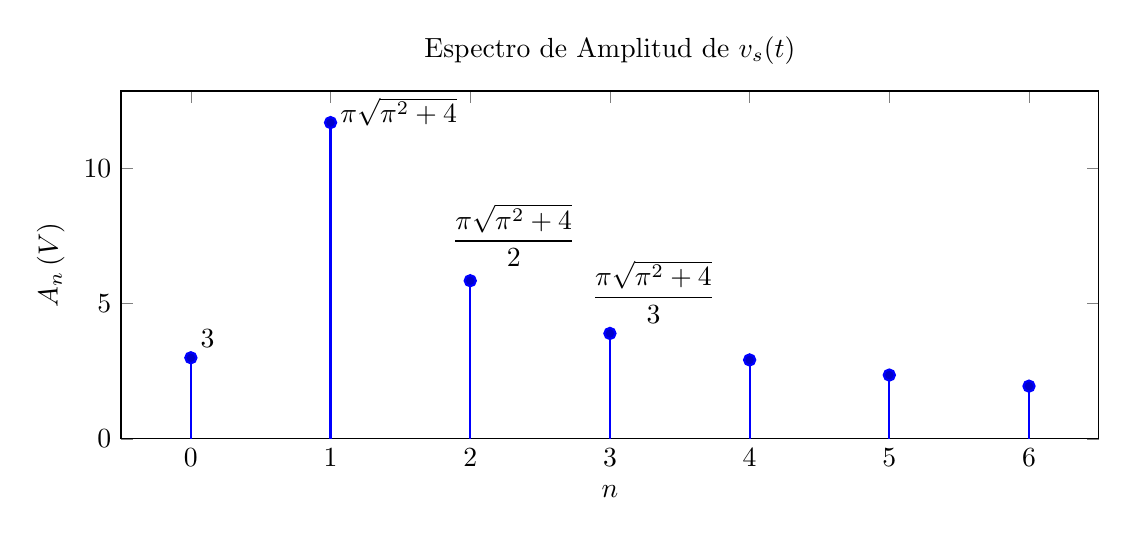
\begin{tikzpicture}
	\begin{axis}[
		title={Espectro de Amplitud de $v_s(t)$},
		xlabel={$n$},
		ylabel={$A_n\,(V)$},
		xmin=-0.5, xmax=6.5,
		ymin=0,
		xtick={0,1,2,3,4,5,6},
		width=14cm,
		height=6cm
		]
		
		\addplot+[ycomb, thick, mark=*] coordinates {
			(0,3.0)
			(1,11.7)
			(2,5.85)
			(3,3.9)
			(4,2.92)
			(5,2.36)
			(6,1.95)
		};
		
		\node at (axis cs:0,3.0) [anchor=south west] {$3$};
		\node at (axis cs:1,11.2) [anchor=south west] {$\pi\sqrt{\pi^2+4}$};
		\node at (axis cs:1.8,6) [anchor=south west] {$\dfrac{\pi\sqrt{\pi^2+4}}{2}$};
		\node at (axis cs:2.8,3.9) [anchor=south west] {$\dfrac{\pi\sqrt{\pi^2+4}}{3}$};
		
	\end{axis}
\end{tikzpicture}

\end{document}
